%%%%%%%%%%%%%%%%%%%%%%%%%%%%%%%%%%%%%%%%%%%%%%%%%%%%%%%%%%%%%%%%
\chapter{Balança Digital}
Para o desenvolvimento deste projeto, foi criado um kit de desenvolvimento para facilitar sua implementação, testes, assim como a execução de alterações e melhoramentos.
\\
\\
Por analise à \textit{figura} \ref{Kit_Desenvolvimento_2}, pode-se verificar a montagem em esqueleto do equipamento,
\begin{figure}[H]
	\centering
	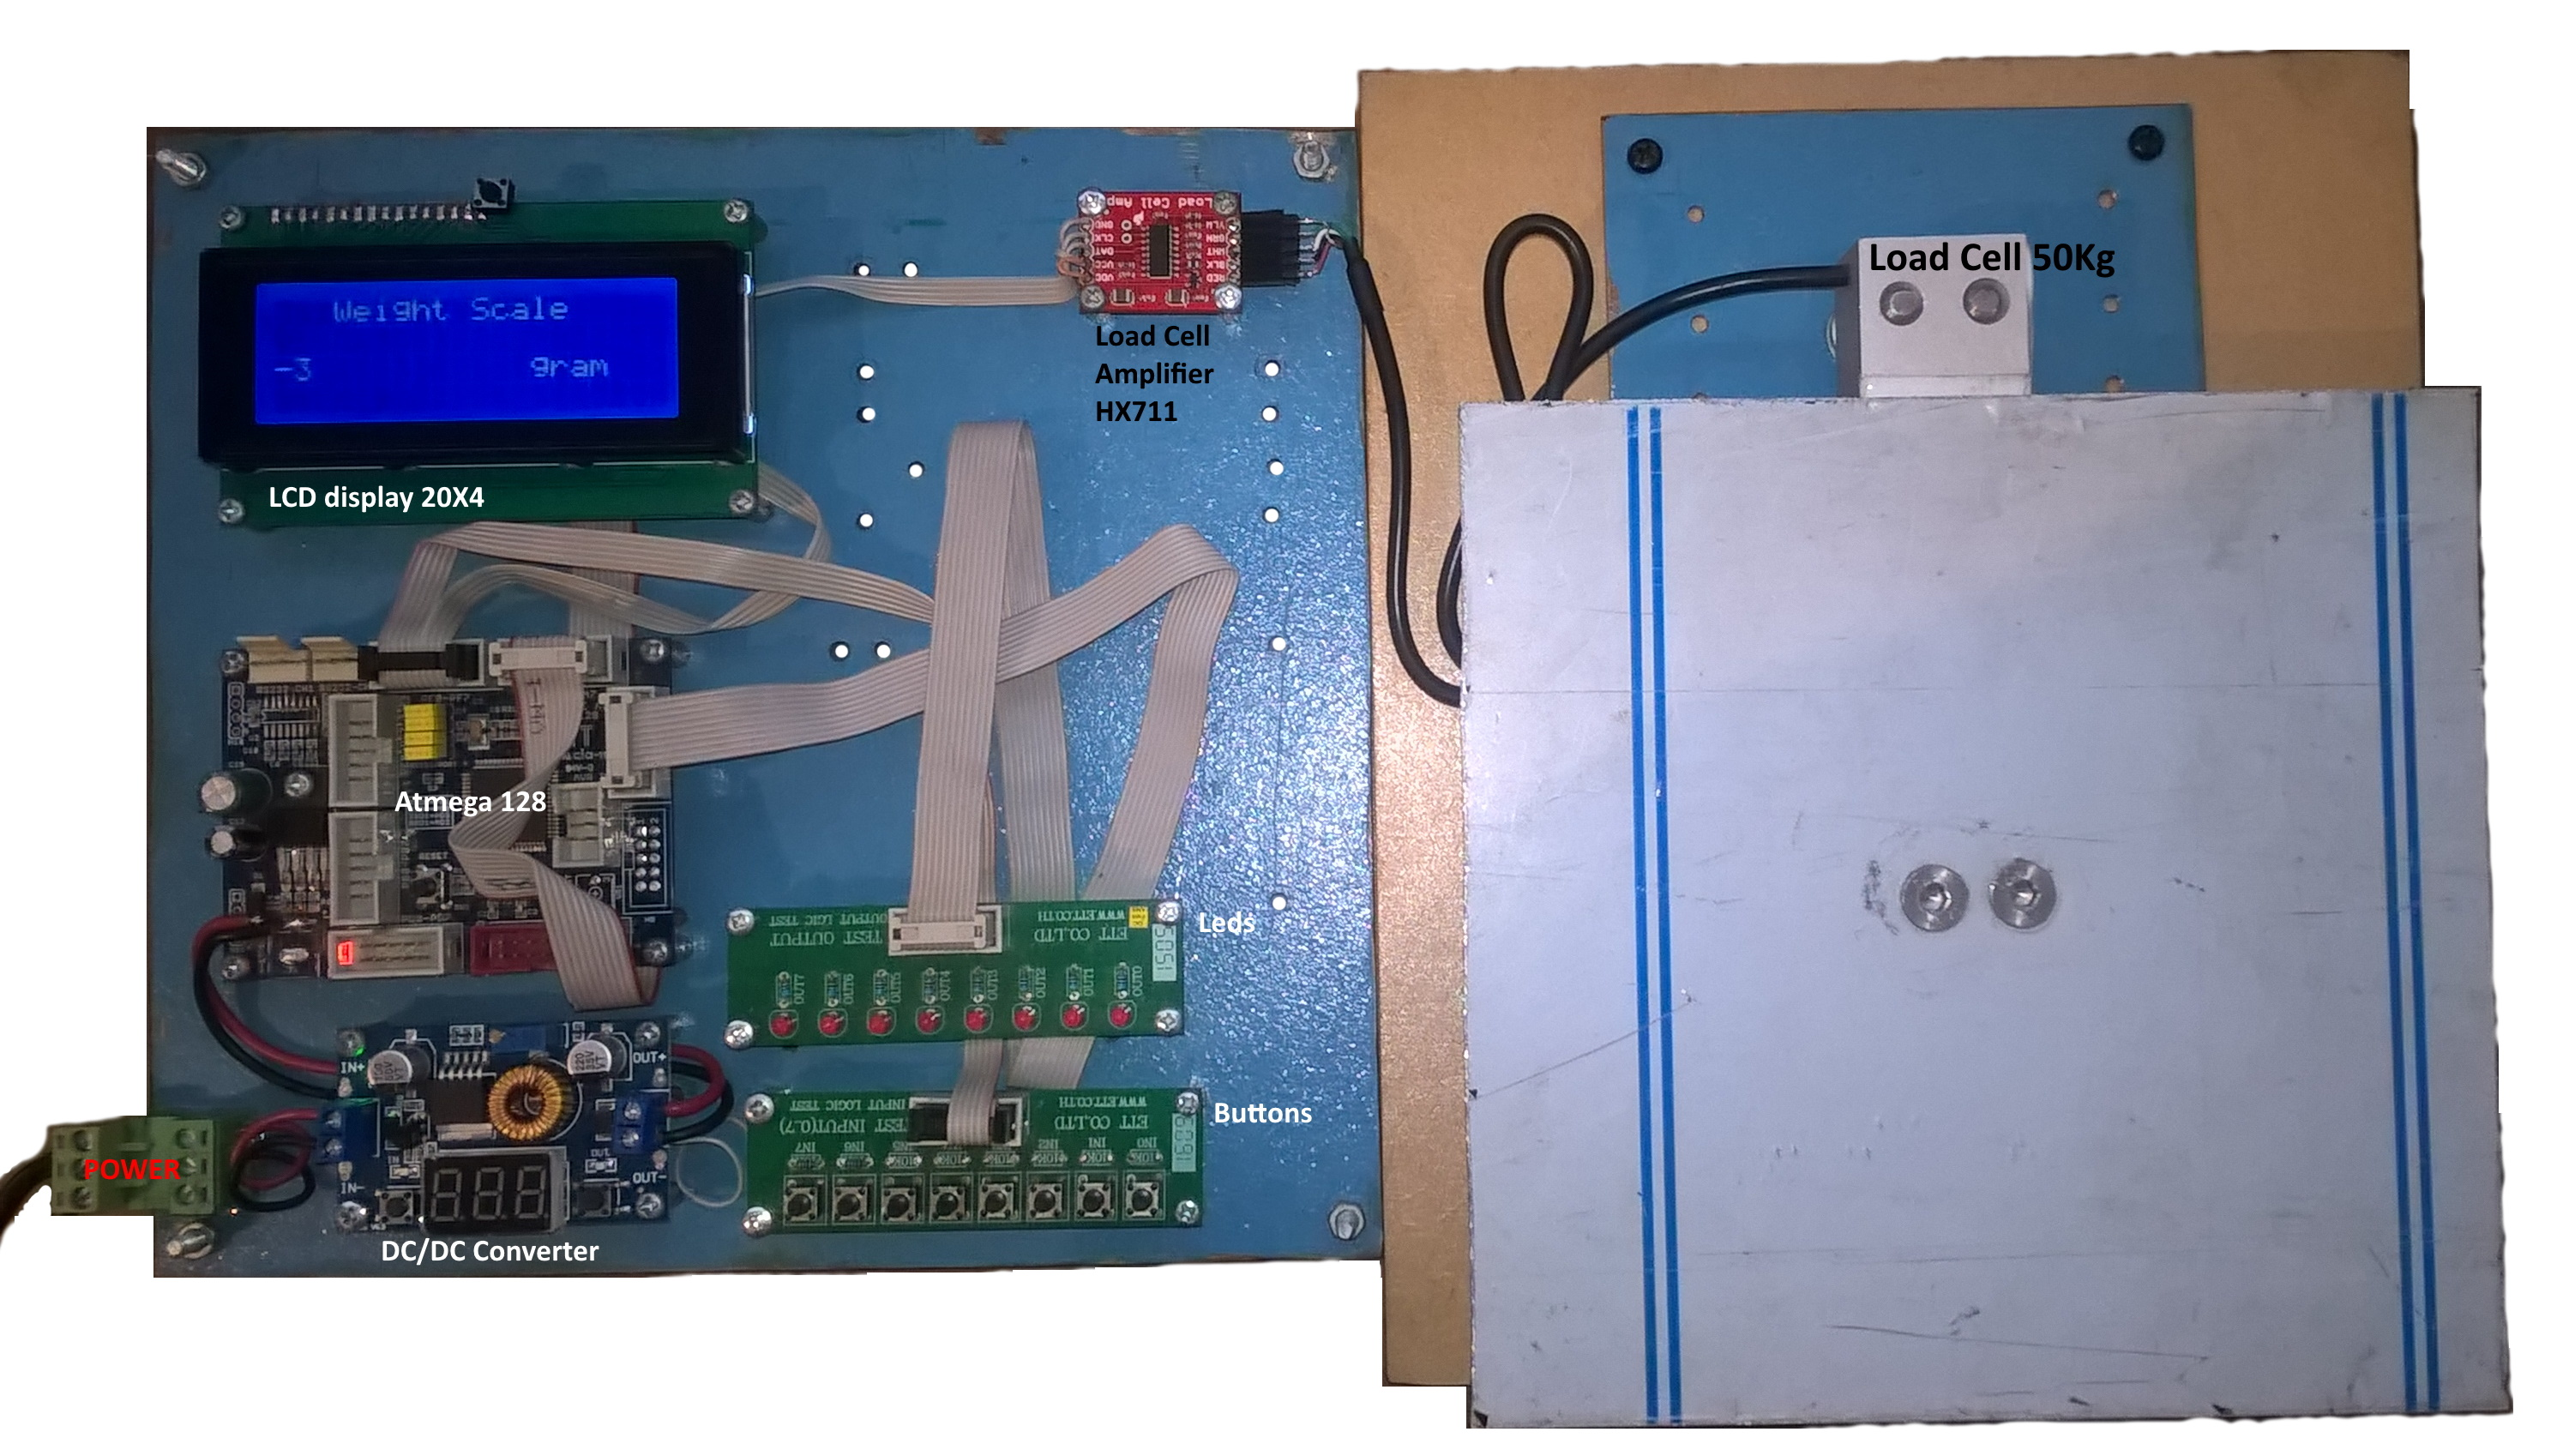
\includegraphics[scale=0.12]{./image/PESTA/kit/Kit_Desenvolvimento_2.jpg}
	\caption{Kit de Desenvolvimento}
	\label{Kit_Desenvolvimento_2}
\end{figure}
a seguir a \textit{figura} \ref{Block_diagram_1} representado os elementos em diagrama de blocos.
\begin{figure}[H]
	\centering
	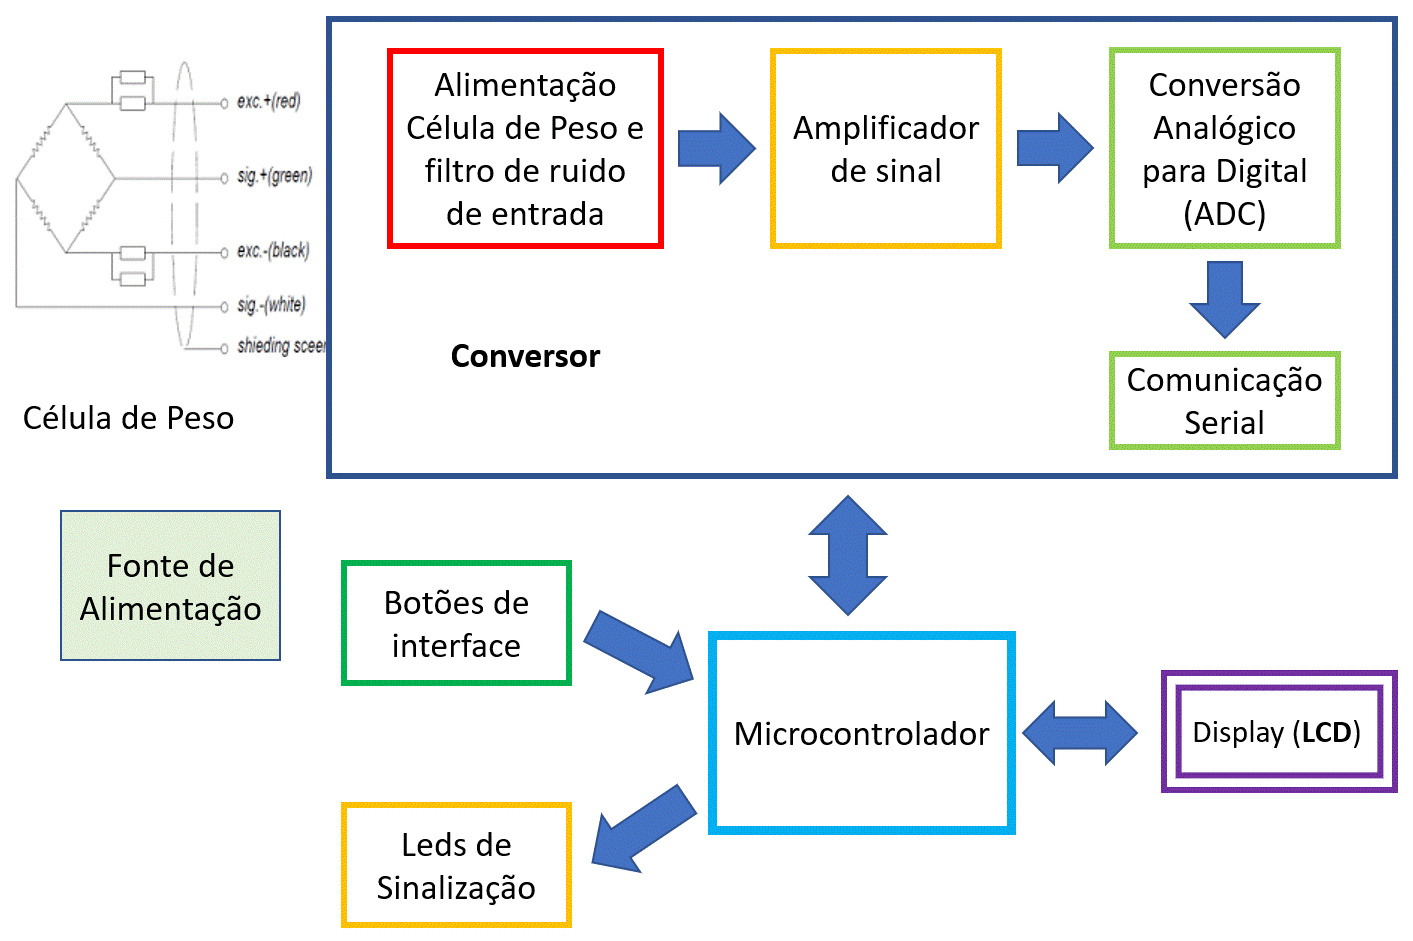
\includegraphics[scale=0.27]{./image/PESTA/Diagrama/Diagrama_bloco_3.jpg}
	\caption{Diagrama Blocos}
	\label{Block_diagram_1}
\end{figure}
%%%%%%%%%%%%%%%%%%%%%%%%%%%%%%%%%%%%%%%%%%%%%%%%%%%%%%%%%%
\section{sensor}
Para medir a massa, recorreu-se a uma \textbf{célula de carga}, que determina a pressão exercida por um dado objeto, neste caso, os sensores (\textit{strain gauges}) são instalados sobre um bloco de alumínio como indicado na \textit{figura} \ref{Load_Cell_1}. A célula de carga utiliza sensores Piezoresistivos numa montagem em ponte \textit{wheatstone}, sobre essa superfície em locais específicos.
\\
\begin{figure}[H]
	\captionsetup{justification=raggedright,singlelinecheck=false}
	\flushleft
	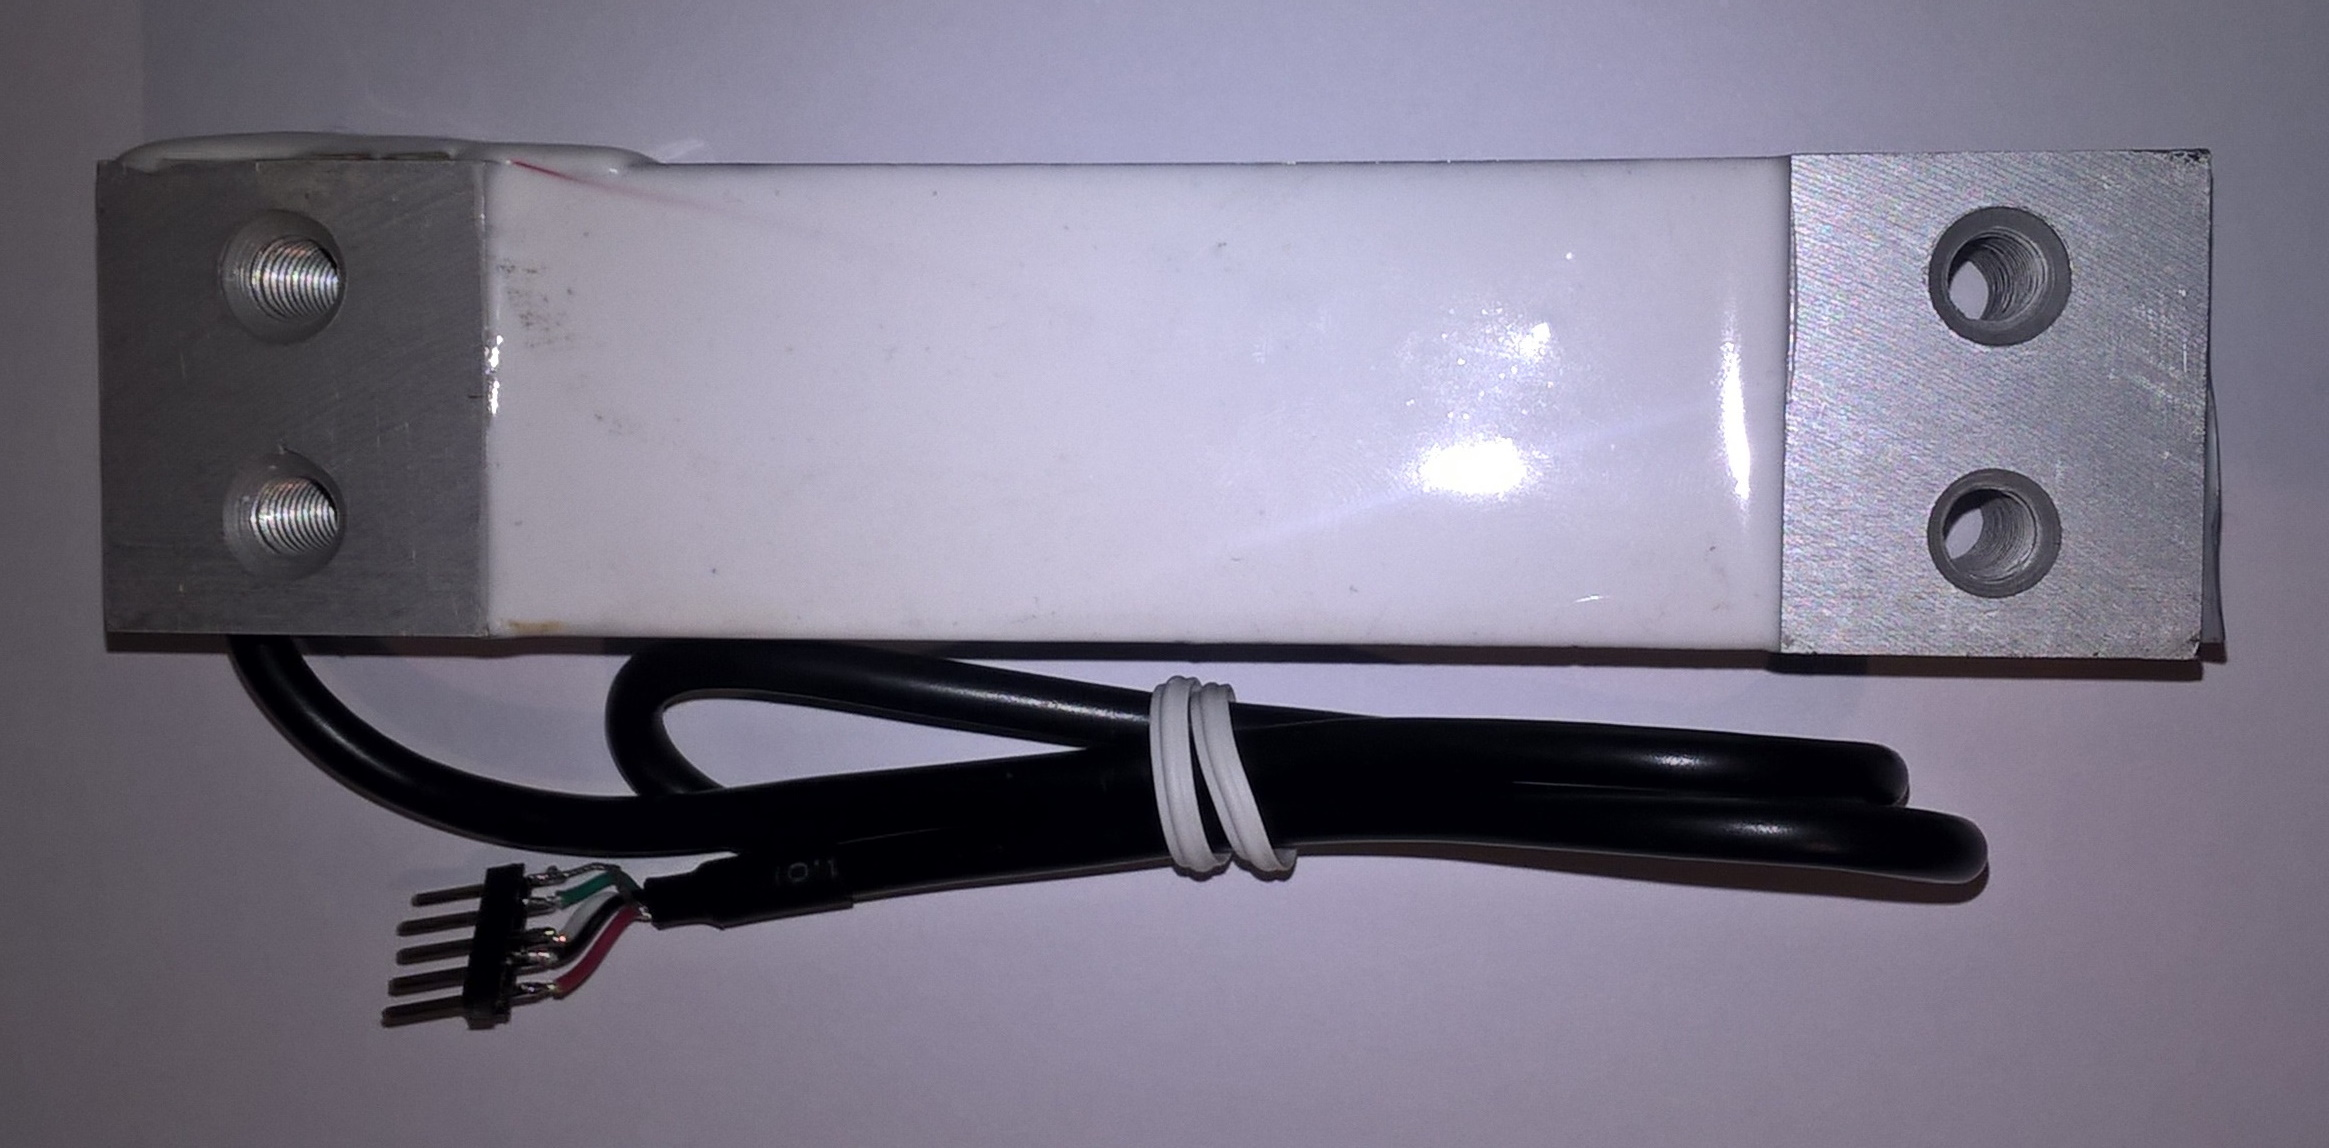
\includegraphics[scale=0.15]{./image/PESTA/material/Load_Cell_1.jpg}
	\caption{Célula de Carga 50Kg}
	\label{Load_Cell_1}
\end{figure}
\figurespace{.5}
O termo Piezoresistividade deriva do seu nome da palavra grega \textit{piezin}, que significa "pressionar". É um efeito exibido por vários materiais que sofrem uma mudança na resistividade devido a uma pressão aplicada. O efeito foi descoberto pela primeira vez por Lord Kelvin em \textcolor{blue}{1856}, que notou que a resistência dos fios de cobre e ferro aumentava quando em tensão mecânica. Ele também observou que os fios de ferro apresentavam uma alteração maior na resistência do que os de cobre. A primeira aplicação do efeito piezoresistivo não apareceu até a década de \textcolor{blue}{1930}, cerca de \textcolor{blue}{75} anos após a descoberta de Lord Kelvin. Em vez de usar fios de metal, esses assim chamados medidores de tensão mecânica, são geralmente feitos de uma folha de metal fina, montada em uma película de suporte, que pode ser colada em uma superfície. O sensor de fita de metal típico é representado na \textit{figura} \ref{strain_gauge_1} \cite{book-9}.
\\
\\
\begin{minipage}[!b]{.5\linewidth}
\begin{figure}[H]
	\captionsetup{justification=raggedright,singlelinecheck=false}
	\flushleft
	\figurespace{1}
	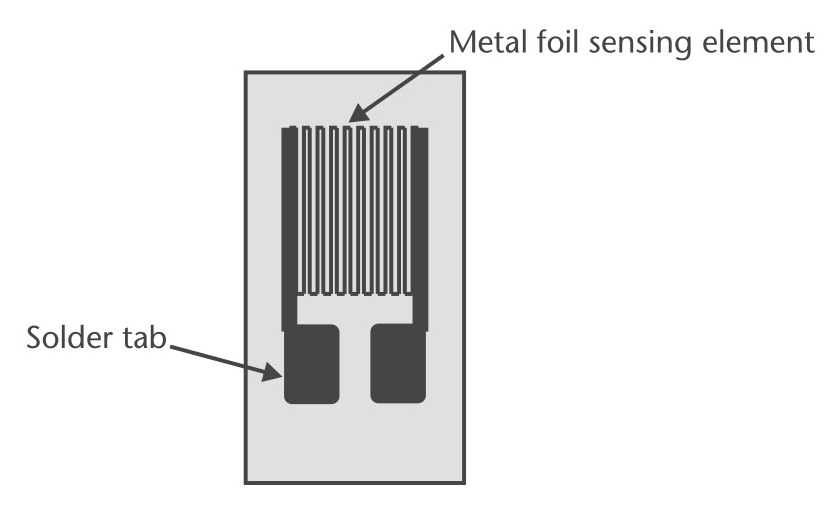
\includegraphics[height=4cm]{./image/PESTA/general/strain_gauge_1.jpg}
	\caption{Fita metálica \textit{strain gauge} \cite{book-9}}
	\label{strain_gauge_1}
\end{figure}
\end{minipage}
\begin{minipage}[!b]{.5\linewidth}
\begin{figure}[H]
	\captionsetup{justification=raggedright,singlelinecheck=false}
	\flushleft
	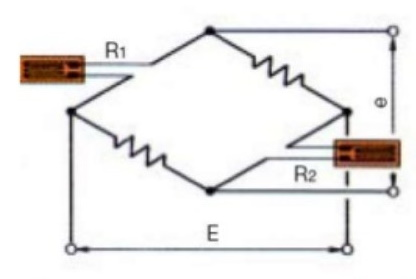
\includegraphics[height=5cm]{./image/PESTA/schematic/Wheatstone_2.jpg}
	\qquad \caption{Ponte \textit{Wheatstone}}
	\label{wheatstone_2}
\end{figure}
\end{minipage}
\minipagespace{.5}
\begin{minipage}[!b]{.4\linewidth}
	\begin{figure}[H]
		\captionsetup{justification=raggedright,singlelinecheck=false}
		\flushleft
		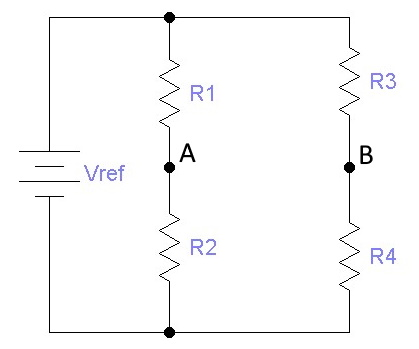
\includegraphics[height=5cm]{./image/PESTA/schematic/Wheatstone_1.jpg}
		\caption{\textit{Wheatstone} por resistências \cite{book-10}}
		\label{wheatstone_1}
	\end{figure}
\end{minipage}
\begin{minipage}[!b]{.6\linewidth}
	\setlength{\jot}{10pt}% tweak
	\begin{align}
		\label{eq:wheatstone}
		&V_A =  \frac{R_2}{R_1 + R_2} \; V_{ref} \; , \; V_B=\frac{R_4}{R_3 + R_4} \; V_{ref} \\
		&V_{AB} =  V_A - V_B = e \\
		&V_{AB}= \left(\frac{R_2}{R_1 + R_2} - \frac{R_4}{R_3 + R_4}\right) \; Vref \\
		&e = \frac{R_2 R_3 - R_4 R_1}{(R_1 + R_2)(R_3 + R_4)} \; Vref
	\end{align}
	\minipagespace{.01}
\end{minipage}
\minipagespace{.5}
Normalmente nesta configuração (\textit{wheatstone}, figura \ref{wheatstone_2} e \ref{wheatstone_1}), só é usado um ou dois sensores, e estes podem estar ligados nos extremos opostos, ou ligados ao mesmo ponto da alimentação, só em casos muito raros são utilizados quatro sensores na qual sua sensibilidade é considerada máxima. Se o valor das quatro resistências são iguais ou nos casos em que [$R_2 R_3 = R_4 R_1$], então a tensão $V_{AB}$ na saída é nula.
\\
\\
Para perceber melhor o funcionamento do sensor \textit{\textbf{strain gauge}} é aconselhável recorrer a literatura \cite{book-9} e \cite{book-10}, que explica como são feitas, seus dimensionamentos e processos de fabrico.
\newpage
A montagem da mesa (prato) de medição  esta demonstrado na \textit{figura} \ref{Prato},
\minipagespace{5}
\begin{minipage}[!b]{\linewidth}
\begin{figure}[H]
	\centering
	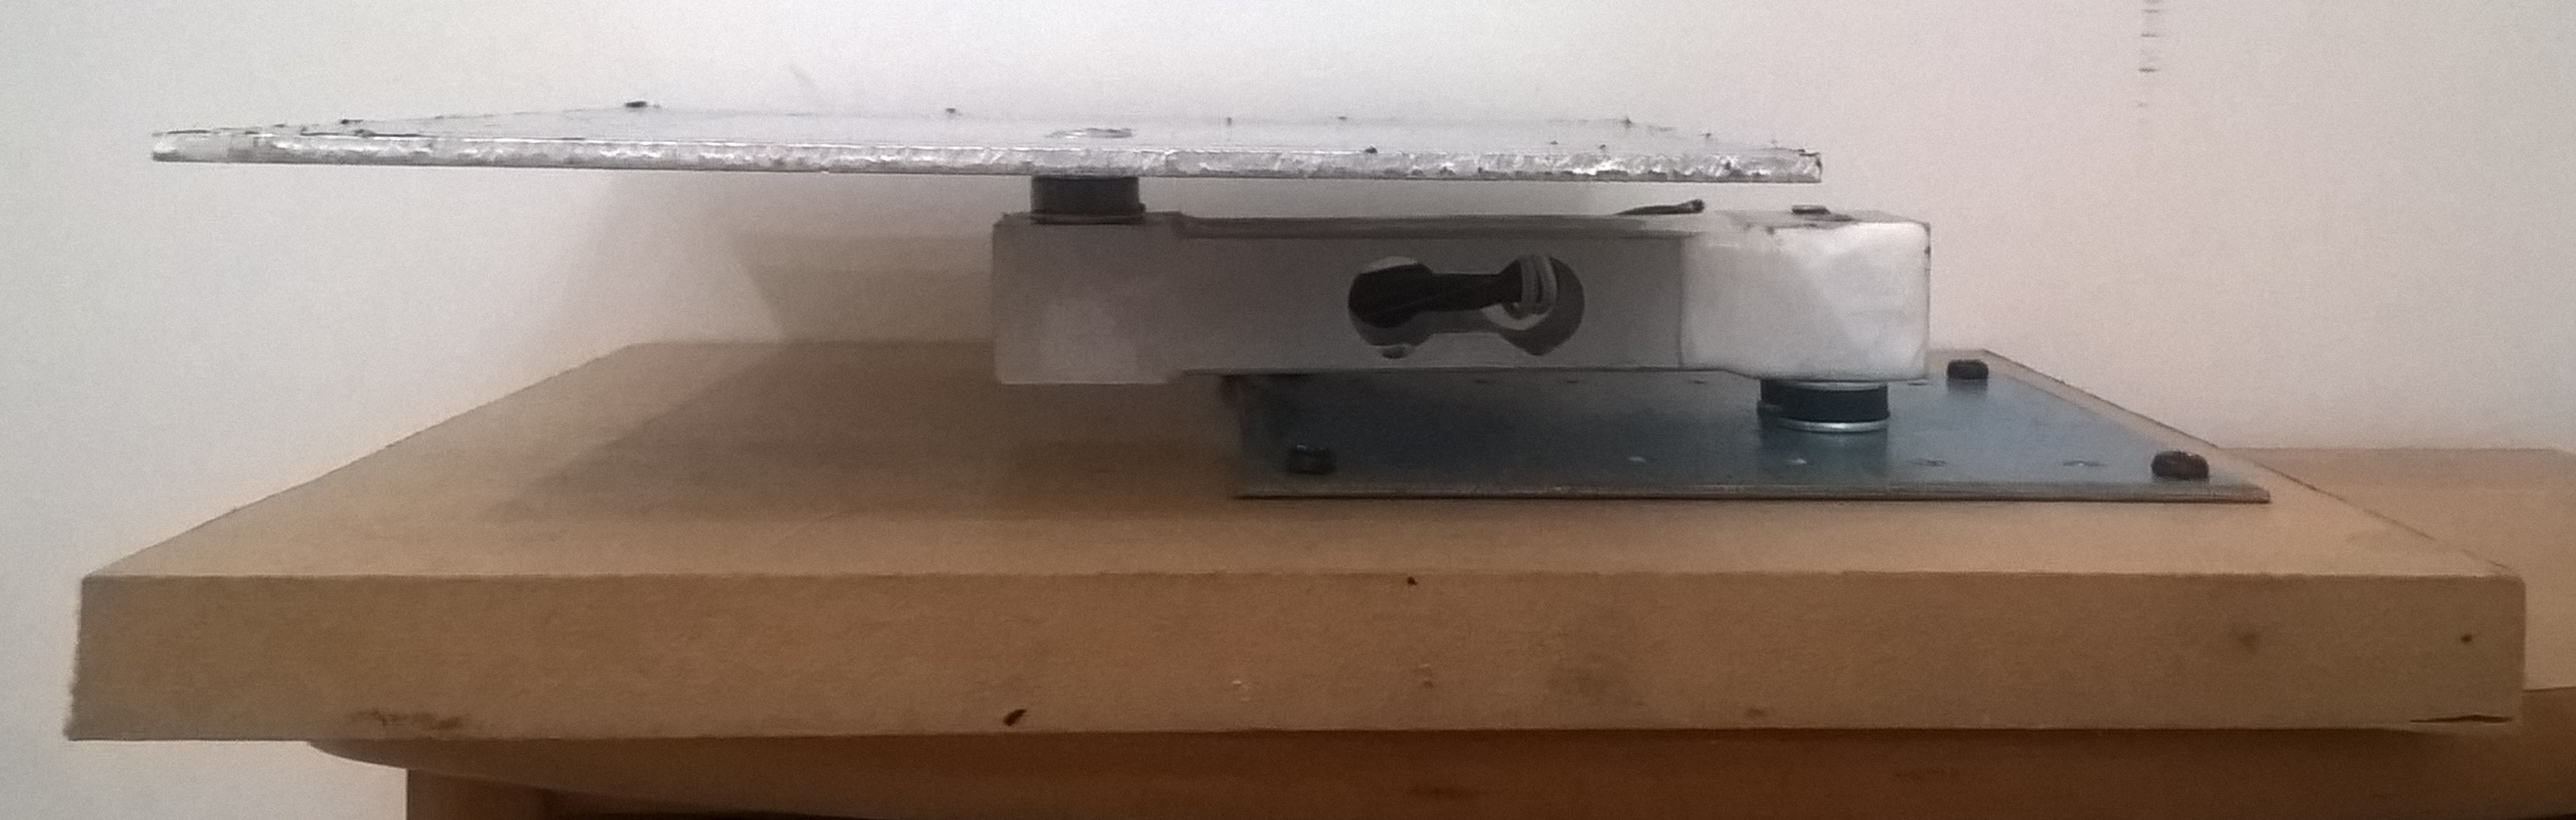
\includegraphics[scale=0.16]{./image/PESTA/material/Prato.jpg}
	\caption{Prato}
	\label{Prato}
\end{figure}
\end{minipage}
\newpage
%%%%%%%%%%%%%%%%%%%%%%%%%%%%%%%%%%%%%%%%%%%%%%%%%%%%%%%%%%
\section{Amplificador de sinal}
A amplificação é geralmente um requisito fundamental, pois a maioria dos sensores, tendem a produzir níveis de sinal significativamente mais baixos, do que aqueles usados no processador digital. Sensores resistivos podem precisar de um amplificador para a célula de carga. Se possível, é vantajoso ter o ganho o mais próximo possível do elemento sensor. Em situações onde um maior ganho é necessário, muitas vezes pode haver implicações para lidar com quaisquer efeitos adversos, como o ruído, problemas de \textit{layout} do \textit{chip}, os transitórios agudos associados aos sinais digitais que precisam de ser mantidos bem longe dos circuitos analógicos \textit{front-end}. \cite{book-9}
\\
\\
A ligação destes componentes é intuitivo e fácil de se perceber, o que é complexo neste trabalho é a interligação destes equipamentos com o micro controlador por meio de \textit{software} e criar o \textit{driver} de comunicação para a placa do amplificador de sinal (\textit{chip} HX711 figura \ref{HX711_Schematic_1}), já que o protocolo de comunicação é proprietário.
\\
\\
\begin{figure}[H]
	\captionsetup{justification=raggedright,singlelinecheck=false}
	\centering
	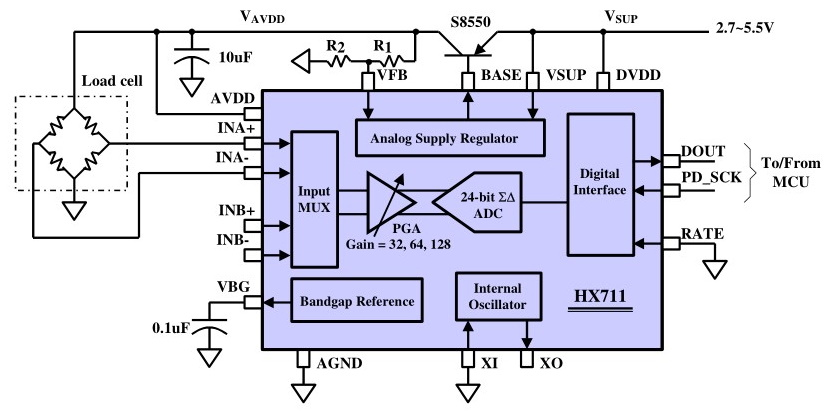
\includegraphics[scale=0.35]{./image/PESTA/schematic/HX711_Schematic_1.jpg}
	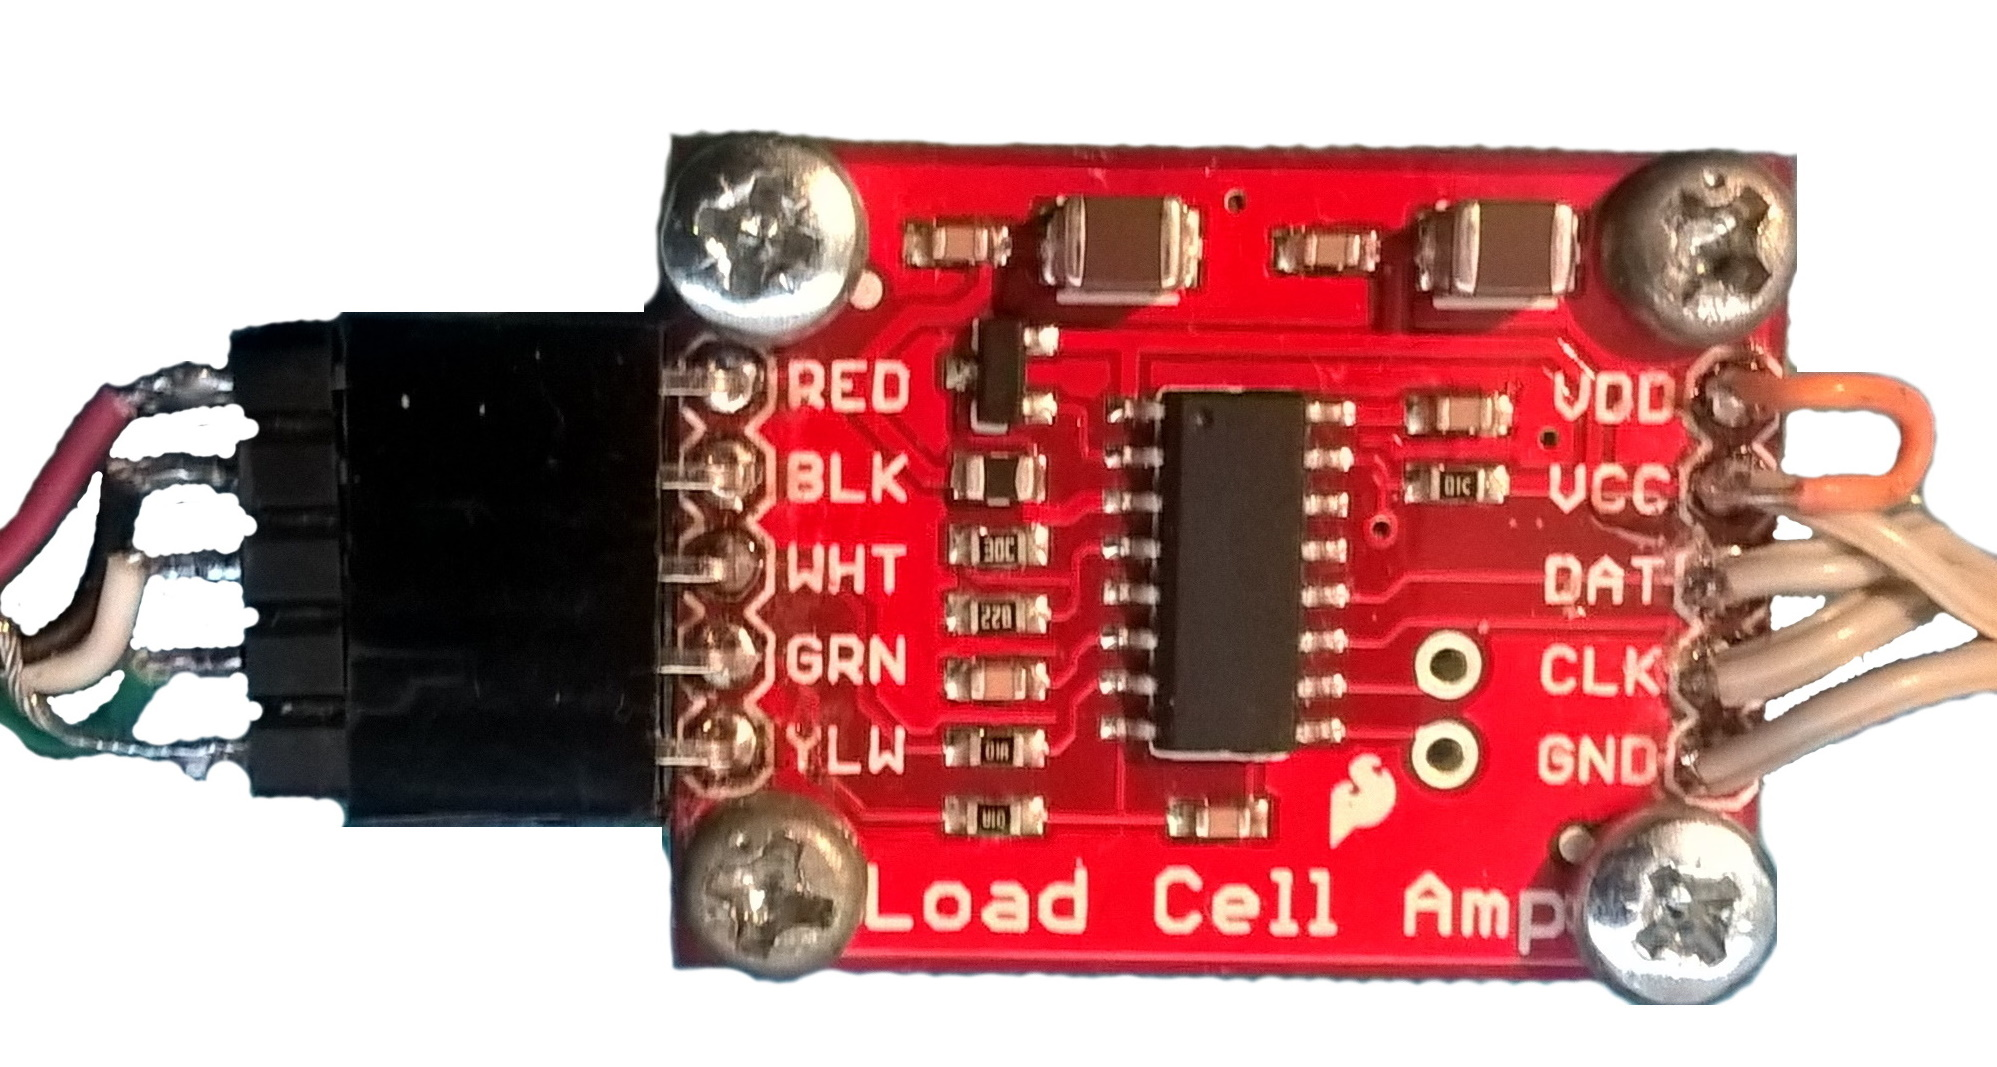
\includegraphics[scale=0.1]{./image/PESTA/material/HX711_board_1.jpg}
	\caption{Amplificador de Sinal [HX711]}
	\label{HX711_Schematic_1}
\end{figure}
\figurespace{.5}
A placa \textit{Load Cell Amplifier } pode ser programada fisicamente, para determinar o numero de amostras por segundo a ser transmitido. Este circuito tem duas opções; a opção de \textcolor{blue}{10} amostras por segundo, e de \textcolor{blue}{80} amostras. Neste projeto optei pela segunda opção que necessita de uma pequena configuração na placa de circuito de impresso, isto é, é necessário abrir o \textit{jumper} respetivo de configuração.
\\
\\
\begin{table}[H]
	\centering
	\caption{Terminais HX711 ({\tiny \scriptsize{top view}})}
	\begin{tabular}{||L{1cm} C{3cm} | p{3cm}  C{2cm}||}
		\hline
		\multicolumn{2}{||c|}{MCU} & \multicolumn{2}{|c||}{\textit{Célula de peso}}\\ [1ex]
		\hline
		1 & GND & EARTH (GND) & YLW \\ 
		2 & CLK & INPA & GRN \\
		3 & DATA & INNA & WHT \\
		4 & VCC &  GND & BLK \\
		5 & VDD & $V_{ADC}$ & RED \\ [1ex]
		\hline
	\end{tabular}	
	\label{HX711_connection}
\end{table}
\tablespace{.3}
A conversão de informação acontece na transição entre o sinal continuo da vida real, para um sinal discreto associado ao mundo digital. Tipicamente esta etapa consiste na conversão de um sinal analógica para digital.
\\
O processamento digital pode consistir no processamento de rotinas para compensar os desvios por linearização, a sensibilidade e o \textit{offset}, ou o processamento de técnicas mais sofisticadas como reconhecimento de padrões, (tais como, redes neuronais) para equipamentos de sensores vetoriais.\cite{book-9}
\\
A comunicação é responsável por criar rotinas necessárias para transferir e receber a informação e sinais de controle, entre o sensor e o processador, que toma lugar como componente central, tratando a informação, guardando os dados e fazendo rotinas, tais como, rotinas de calibração, rotinas de teste e controlo de ganho da amplificação. \cite{book-9}
\\
\\
\begin{figure}[H]
	\centering
	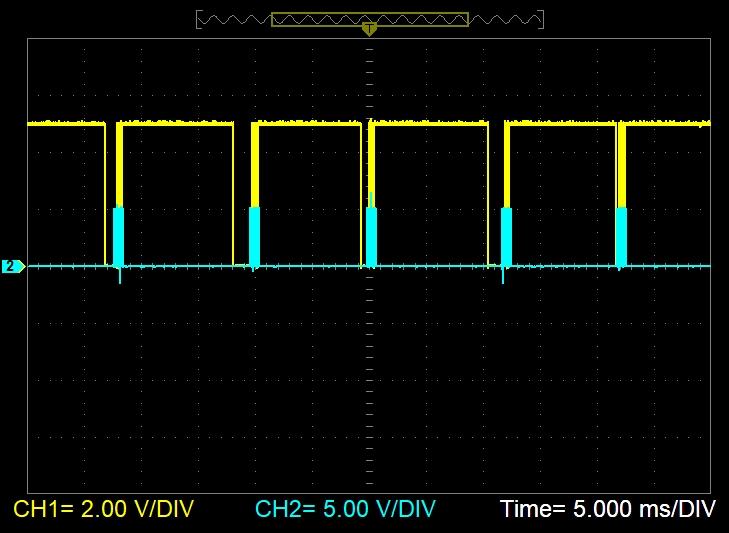
\includegraphics[scale=0.55]{./image/PESTA/graph/80SPS64GAIN/SPS_80.JPG}
	\caption{Amostras}
	\label{SPS_64}
\end{figure}
\figurespace{.5}
A livraria (\textit{driver}) do integrado HX771, recorre a interrupções periódicas, e quando a linha de sinal da informação vai para a massa esta  indica que tem um pacote de leitura pronto a ser transmitido.
\\
\\
\begin{minipage}[!b]{\linewidth}
\begin{minipage}[!b]{.40\linewidth}
	\begin{table}[H]
		\captionsetup{justification=raggedright,singlelinecheck=false}
		\caption{Configuração Ganho}
		\begin{tabular}{ | c | c | c |  }
			\hline
			\makecell[c]{PD\_SCK \\ Impulsos} & Entrada  & Ganho \\
			\hline
			\hline
			25 & \textbf{A} & 128 \\
			\hline
			26 & \textbf{B} & 32 \\
			\hline
			27 & \textbf{A} & 64 \\
			\hline
		\end{tabular}
		\label{Gain_Selection}
	\end{table}
	\tablespace{2.5}
\end{minipage}
\begin{minipage}[l]{.6\linewidth}
\vspace{.3cm}
Como indicado abaixo no gráfico, em que a linha \textcolor{yellow}{amarela} é a informação, e a linha \textcolor{BlueGreen}{azul} o respetivo \textit{clock} que é gerado pelas interrupções do micro-controlador, fazendo um deslocamento dos \textcolor{blue}{24} \textit{bits}, que por fim transmite para o amplificador, o ganho de amplificação a ser usado pelo numero excedente de \textit{clock cycles}, em que nesta demonstração da \textit{figura} \ref{Gain_128_example} é \textcolor{blue}{um}, e corresponde a um ganho de \textcolor{blue}{128}, respeitando a informação apresentada na \textit{tabela} \ref{Gain_Selection},  e de seguida o exemplo da \textit{figura} \ref{Gain_64_example}, com um ganho de \textcolor{blue}{64}, pois tem \textcolor{blue}{três} impulsos excedentes.
\end{minipage}
\end{minipage}
\\
\begin{minipage}[!b]{\linewidth}
\begin{minipage}[!b]{.43\linewidth}
\begin{figure}[H]
	\captionsetup{justification=raggedright,singlelinecheck=false}
	\flushleft
	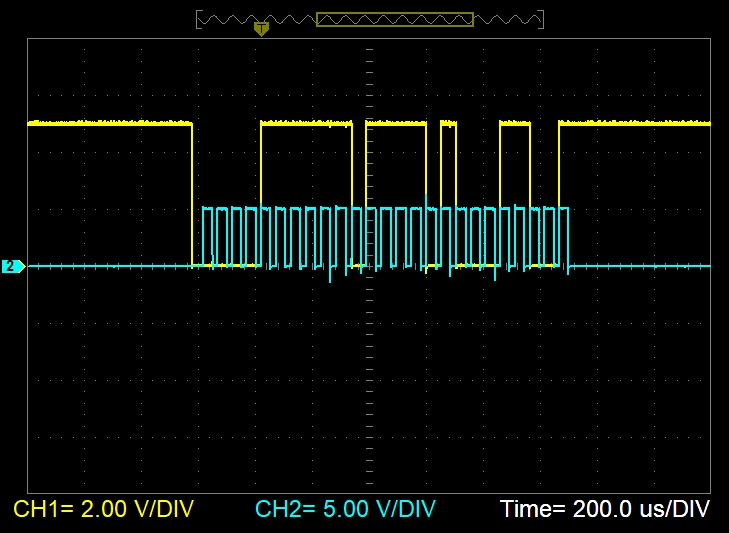
\includegraphics[scale=0.3]{./image/PESTA/graph/80SPS128GAIN/Gain_128_example.JPG}
	\caption{Ganho de 128}
	\label{Gain_128_example}
\end{figure}
\end{minipage}
\hspace{1cm}
\begin{minipage}[!b]{.43\linewidth}
\begin{figure}[H]
	\captionsetup{justification=raggedright,singlelinecheck=false}
	\flushleft
	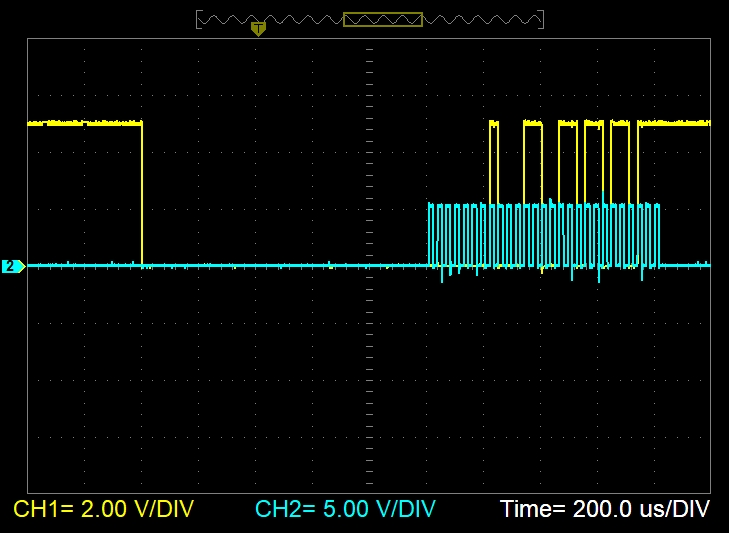
\includegraphics[scale=0.3]{./image/PESTA/graph/80SPS64GAIN/Gain_64_example.JPG}
	\caption{Ganho de 64}
	\label{Gain_64_example}
\end{figure}
\end{minipage}
\end{minipage}
\minipagespace{.3}
Para obter este resultado, a livraria \textit{driver} para o \textit{Load Cell Amplifier} teve de ter em consideração que a arquitetura do micro-controlador é de \textcolor{blue}{8} \textit{bits}, uma vez que a estrutura do pacote de informação é entre \textcolor{blue}{25} a \textcolor{blue}{27} impulsos do \textit{clock cycle} em que é transmitido primeiro o \ac{msb}.
\\
\\
O código que executa esta rotina é demonstrado na \textit{lista} \ref{HX711-read-raw}, sendo esta chamada pelas interrupções periódicas, e só é ativa quando o resultado da função na \textit{lista} \ref{Main-While-case-1} \textbf{hx.query(\&hx)} é verdadeira.
{
	\lstinputlisting[language=C, caption={função de chamada \textbf{hx.query(\&hx)}}, captionpos=b, label=Main-While-case-1]{./input/code/hx_query.c}
}
\newpage
{
	\lstinputlisting[language=C, caption=HX711\_read\_raw, captionpos=b, label=HX711-read-raw]{./input/code/HX711_read_raw.c}
}
%\listingspace{.1}
Após obter um numero determinado de valores discretos lidos pelo amplificador de sinal (HX711) é calculado uma média,
\begin{equation}
	\label{eq:Mean}
	\overline{x}  =  \frac{1}{n}\sum_{i=1}^n x_i
\end{equation}
para ser tratado e deduzido o valor correspondente da massa.
\newpage
%%%%%%%%%%%%%%%%%%%%%%%%%%%%%%%%%%%%%%%%%%%%%%%%%%%%%%%%%%
\section{Display \acs{lcd}}
O \ac{lcd} utilizado é de 4x20, isto é, quatro linhas de vinte caracteres cada, tornando-se no interface humano principal, e também durante o projeto numa ferramenta extremamente útil para fazer \textit{debug} e executar testes ao código.
\\
\\
Uma livraria já feita para outros projetos serviu para aplicar também neste, poupando bastante tempo, revelando a importância de documentar os conhecimentos adquiridos. A livraria ou se preferem \textit{driver} esta presente no \textit{anexado} \ref{lcd-h} e \ref{lcd-c}.
%[\ref{codigo}]
\\
\\
Abaixo está a tabela \ref{LCD_connections}, com as respetivas ligações, e uma imagem de um \acs{lcd} 4x20 azul na \textit{figura} \ref{4x20_LCD}.
\tablespace{.2}
\begin{table}[H]
	\centering
	\caption{Conexões \acs{lcd}}
	\begin{tabular}{||p{1cm} p{2cm} p{4cm} | p{1cm}||} 
		\hline
		\multicolumn{3}{||c|}{\textbf{LCD Pin}} & \multicolumn{1}{|c||}{\textbf{MCU Pin}}\\ [1ex]
		\hline
		1 & VSS & GND & \\
		2 & VCC & +5V & \\
		3 & VEE & \textit{Contrast Control} & \\
		4 & RS & \textit{Register Select} & Pin 0 \\
		5 & RW & \textit{Read/Write} & Pin 1 \\
		6 & E & \textit{Enable} & Pin 2 \\
		7 & Do & \textit{Data Pin 0} & \\
		8 & D1 & \textit{Data Pin 1} & \\
		9 & D2 & \textit{Data Pin 2} & \\
		10 & D3 & \textit{Data Pin 3} & \\
		11 & D4 & \textit{Data Pin 4} & Pin 4 \\
		12 & D5 & \textit{Data Pin 5} & Pin 5 \\
		13 & D6 & \textit{Data Pin 6} & Pin 6 \\
		14 & D7 & \textit{Data Pin 7} & Pin 7 \\
		15 & LED+ & \textit{Led +5V} &  \\
		16 & LED- & \textit{Led Ground} & \\
		\multicolumn{3}{||c|}{\textit{Reboot} \acs{lcd}} & \multicolumn{1}{|l||}{Pin 3}\\ [1ex]
		\hline
	\end{tabular}	
	\label{LCD_connections}
\end{table}
\begin{figure}[H]
	\centering
	%%\captionsetup{justification=raggedright,singlelinecheck=false}
	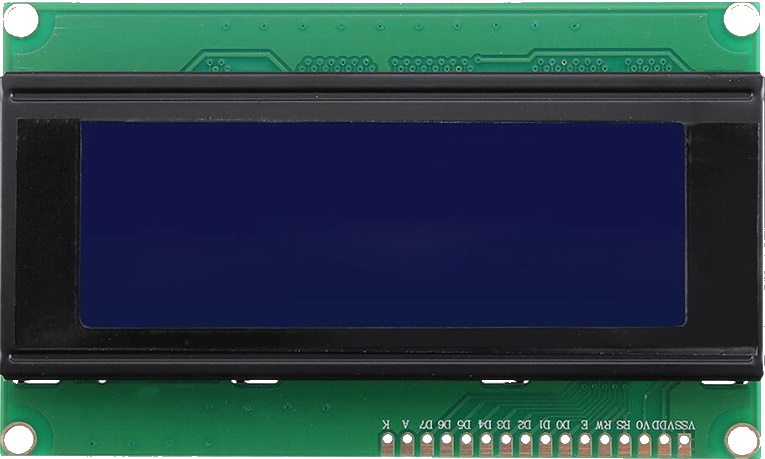
\includegraphics[height=6cm]{./image/PESTA/material/4x20_LCD.jpg}
	\caption{\acs{lcd}}
	\label{4x20_LCD}
\end{figure}
\newpage
%%%%%%%%%%%%%%%%%%%%%%%%%%%%%%%%%%%%%%%%%%%%%%%%%%%%%%%%%%
\section{Micro-controlador}
Os micro-controladores da \textbf{Atmel} de 8 a 32 \textit{bits} são baseados na arquitetura avançada de \textbf{Harvard} na qual está concebido para baixos consumos e performance.
\\
\\
Este tipo de arquitetura tem dois  \textit{buses} (barramentos), um dedicado à leitura das instruções a executar e outra para a escrita e leitura de dados (informação ou dados), isto assegura que uma nova instrução pode ser executada em cada ciclo de relógio, em que elimina todos os estados de espera, quando não ha instruções prontas a executar.
\\
\\
Nos micro-controladores do \ac{avr}, os barramentos estão configurados de forma a dar prioridade ao barramento das instruções do \ac{cpu} acesso à memoria flash, enquanto o barramento da \acs{cpu} de dados tem prioridade de acesso à \ac{sram}.
\\
\\
O espaço de memoria de dados é dividida em três partes, os \ac{gpr} as \ac{sfr} ou memoria de I/O e a \textit{data} \acs{sram}.
\\
\\
Os micro-controladores da AVR utiliza uma arquitetura de instruções \ac{risc} que reduz a complexidade dos circuitos na codificação de cada instrução.
\\
\\
Dai que os micro-controladores que se baseiam nestes tipos de arquitetura são sinonimo de código reduzido, alta performance e baixo consumo energético.
\\
\\
\begin{figure}[H]
	\centering
	%%\captionsetup{justification=raggedright,singlelinecheck=false}
	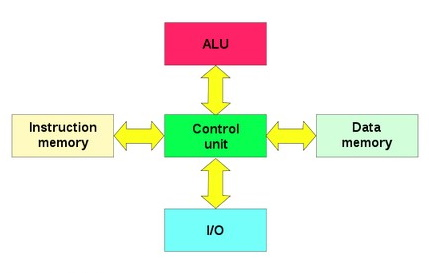
\includegraphics[scale=1]{./image/PESTA/Diagrama/Harvard_architecture.jpg}
	\caption{Harvard Architecture}
	\label{Harvard_architecture}
\end{figure}
\qquad link: \url{https://en.wikipedia.org/wiki/Harvard_architecture}
\newpage
Neste projeto optei pelo Atmega 128 (\textit{figura} \ref{Atmega_128_pinagem}), por ser um dos mais poderosos \ac{mcu} da linha de 8 \textit{bits} da Atmel, e também por estar integrado já numa placa de desenvolvimento dotado de ligações por fichas \ac{idc}, ou seja, utiliza \textit{flat ribbon cables} para ligar os periféricos, o que torna muito mais prático do que sistemas mais atuais, como por exemplo a placa de desenvolvimento Arduino, STMicroelectronics e a \ac{pic} que recorrem a um interface com recurso a pinos (\textit{male pin headers}).
\\
\\
\\
\\
\\
\begin{figure}[H]
	\centering
	%%\captionsetup{justification=raggedright,singlelinecheck=false}
	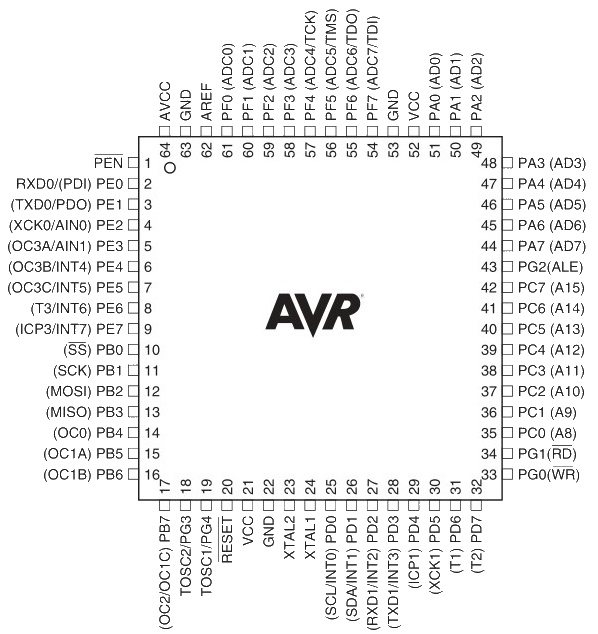
\includegraphics[scale=0.7]{./image/PESTA/material/Atmega128_1.jpg}
	\caption{Atmega 128}
	\label{Atmega_128_pinagem}
\end{figure}
\figurespace{1}
{Transparências Sistemas Digitais 2 \quad \acs{isep} \quad 2008/2009 \quad \textit{link}}:
\\
\url{https://drive.google.com/file/d/1wgOGf8WwYY0OzDhRca9ypXz-iBO55YOF/view?usp=sharing}
\newpage
As características do micro controlador Atmega 128 estão abaixo indicados na lista. Dos componentes que constituem o Atmega 128, os temporizadores são os que considero os mais importantes, o \ac{adc} do \acs{mcu} nem vai ser usado neste projeto, vai ser utilizado um \textit{load cell amplifier} externo, uma alternativa que é muito melhor porque tem maior resolução e especifico para a aplicação em causa.
\\ 
Talvez os \acs{mcu} nem deviam ter a componente \acs{adc} e realçar em meios de comunicação e memoria, tornava-se assim num sistema totalmente digital.
O Atmega 128 é uma escolha acertada para este projeto, considerando as alternativas de optar por um \ac{mcu} de 32 \textit{bits} ou um \textit{embeded system} com sistema operativo integrado, em que no primeiro caso o grau de dificuldade é acrescida devido a ter muito mais configurações e funcionalidades, e a segunda opção de ser exagerada, devido a só utilizar uma muito pequena parte das suas possibilidades, como se diz em inglês um \textit{overkill}, desperdiçando recursos desnecessariamente, e também se iria refletir a nível de custos monetários, no entanto facilita bastante no desenvolvimento de qualquer projeto, pois esta-se a trabalhar sobre uma camada de nível superior.
\\
\\
\begin{minipage}{\linewidth}
{\Large Caracteristicas do Atmega 128 :}
\normalsize
\begin{itemize}	
	\setlength\itemsep{-0.3em}
	\item Arquitectura \acs{risc}
	\item 33 instruções (a maior parte executada num único ciclo de execução)
	\item 32 x 8 registos de trabalho (arquitectura de registos)
	\item Até 16 \acs{mips} (@16MHz) – 62.5ns / instrução
	\item 64K x 16 palavras de programa – 128K bytes FLASH
	\item 4K bytes de \acs{ram} interna
	\item 4K bytes de E2PROM de dados
	\item Ciclos de escrita / leitura – FLASH=10000, E2PROM=100000
	\item 7 Portos de IO \\
		\hspace*{.5cm}	-> 6 x 8 bits (Portos A .. F) \\
		\hspace*{.5cm}	-> 1 x 5 bits (Porto G)
	\item 2 x Timer / Counter de 8 bits
	\item 2 x Timer / Counter de 16 bits
	\item 1 x Real Time Counter ( com oscilador independente)
	\item 2 x \acs{pwm} de 8 bits
	\item 6 x \acs{pwm} de 16 bits
	\item \acs{adc} de 10 bits (8 canais)
	\item 2 x \acs{usart}
	\item \acs{spi}
	\item \acs{twi} (I2C)
\end{itemize}
\end{minipage}
\minipagespace{0.5}
\newpage
Para programar este micro-controlador (\textbf{Atmega 128}), foi utilizado o programador da marca da Atmel, precisamente o \ac{atmel-ice} \textit{figura} \ref{Programador_1}, que para este equipamento tem disponível programação via \ac{isp} \textit{figura} \ref{ISP_6_8_10pin} e \ac{jtag}.
\minipagespace{.2}
\begin{minipage}[!b]{.5\linewidth}
	\begin{figure}[H]
		\captionsetup{justification=raggedright,singlelinecheck=false}
		\flushleft
		\includegraphics[scale=0.75]{./image/PESTA/programador/Atmel_ice.png}
		\caption{KIT \acs{atmel-ice}}
		\label{Programador_1}
	\end{figure}
\end{minipage}
\hspace{.5cm}
\begin{minipage}[!b]{.5\linewidth}
	\begin{figure}[H]
		\captionsetup{justification=raggedright,singlelinecheck=false}
		\flushleft
		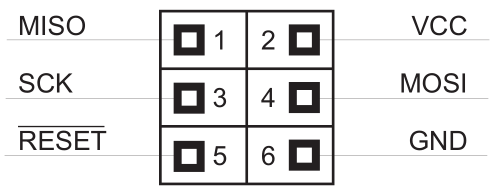
\includegraphics[scale=0.45]{./image/PESTA/programador/isp_6pin.png}
		\hspace{.3cm}
		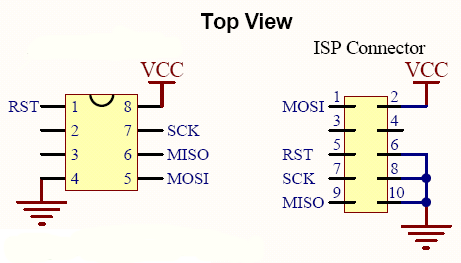
\includegraphics[scale=0.5]{./image/PESTA/programador/isp_8e10pin.png}
		\caption{Fichas \acs{isp}}
		\label{ISP_6_8_10pin}
	\end{figure}
\end{minipage}
%%%%%%%%%%%%%%%%%%%%%%%%%%%%%%%%%%%%%%%%%%%%%%%%%%%%%%%%%%
\section{Fonte de Alimentação}
\begin{minipage}[!b]{.5\linewidth}
	\begin{figure}[H]
		\captionsetup{justification=raggedright,singlelinecheck=false}
		\flushleft
		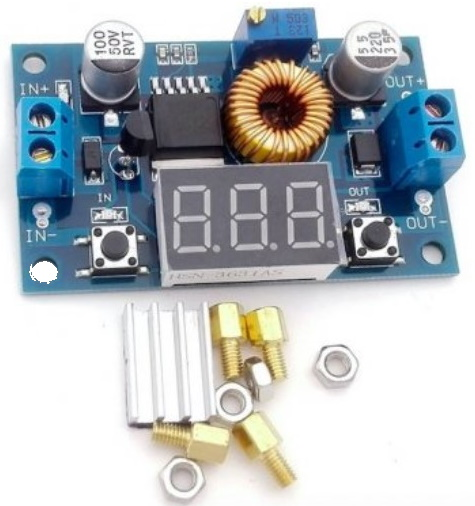
\includegraphics[scale=0.5]{./image/PESTA/material/DCDC_converter.jpg}
		\caption{\textit{Buck Converter}}
		\label{buck-converter}
	\end{figure}
	\figurespace{.1}
\end{minipage}
\begin{minipage}[!b]{.5\linewidth}
\small
Caracteristicas DC/DC:
	\begin{itemize}
		\setlength\itemsep{-0.5em}
		\footnotesize
		\item 5A 75W Conversor Abaixador (\textit{Step-down})
		\item Alimentação Entrada: 4 - 38VDC
		\item Tensão de saída: 1.25 - 36VDC
		\item Corrente saída: 0 - 5A
		\item Potência saída: 75W
		\item Voltímetro: 4 até 40V, erro ±0.1V
		\item \textit{Led} indicadores
		\item Frequência de operação: 180KHz
		\item Eficiência até 96 \%
		\item Proteção Térmica
		\item Limitador de Corrente
		\item Proteção contra curto circuito
		\item NOTA: Não tem proteção de inversão de polaridade
		\item L x W x H = 6.6 x 3.9 x 1.8 CM
		\item Massa: 28g
	\end{itemize}
\end{minipage}
Como a \textit{mainboard} tem um regulador de tensão de 5 Volt, para aumentar a eficiência  e ter uma alimentação variável de entrada utilizo o \textit{buck converter} da \textit{figura} \ref{buck-converter}. Como podemos ver nas características.
%%%%%%%%%%%%%%%%%%%%%%%%%%%%%%%%%%%%%%%%%%%%%%%%%%%%%%%%%%
\chapter{Software}
O \ac{ide} utilizado neste trabalho foi o \textbf{\textit{{Microchip Studio for AVR\textsuperscript{\textregistered} and SAM Devices}}} (\textit{version: 7.0.2542}).
\\
\begin{minipage}[!b]{.55\linewidth}
\begin{figure}[H]
	\captionsetup{justification=raggedright,singlelinecheck=false}
	
\includegraphics[scale=0.6]{./image/PESTA/IDE/Microchip-Studio.png}
	\caption{Microchip Studio}
	\label{Microchip-Studio}
\end{figure}
\end{minipage}
\begin{minipage}[!b]{.45\linewidth}
	Ao lado a figura \ref{Microchip-Studio} nos mostra o logo da empresa, e abaixo a figura \ref{Work-Space} demonstra o ambiente de trabalho onde se executa todo o código que vai correr no micro-controlador.
	\\
	\\
	\\
	\\
	\\
\end{minipage}
\minipagespace{.5}
\begin{figure}[H]
	\centering
	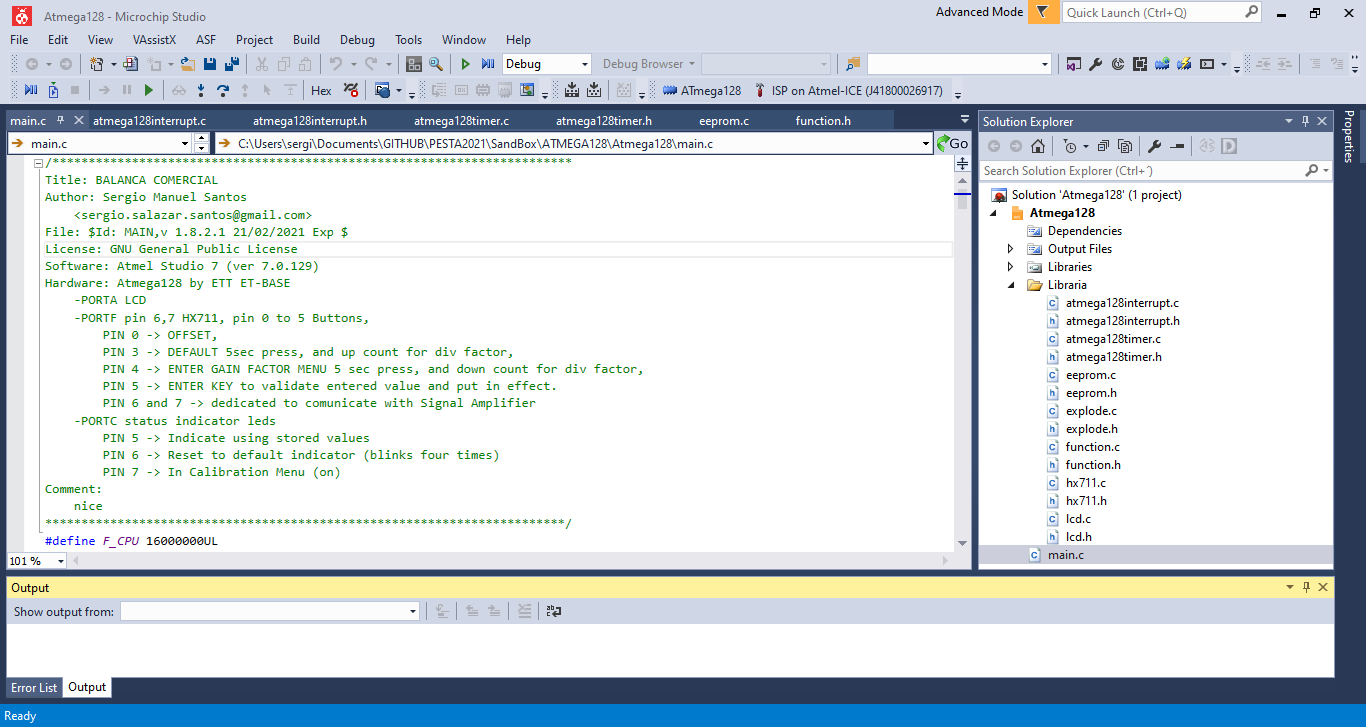
\includegraphics[width=\linewidth]{./image/PESTA/IDE/Work-Space.png}
	\caption{Ambiente de trabalho}
	\label{Work-Space}
\end{figure}
\newpage
 A programação foi feita em Linguagem \textbf{C}, e sua estrutura sintática esta abaixo mencionada:
\\
\\
\begin{figure}[H]
	\centering
	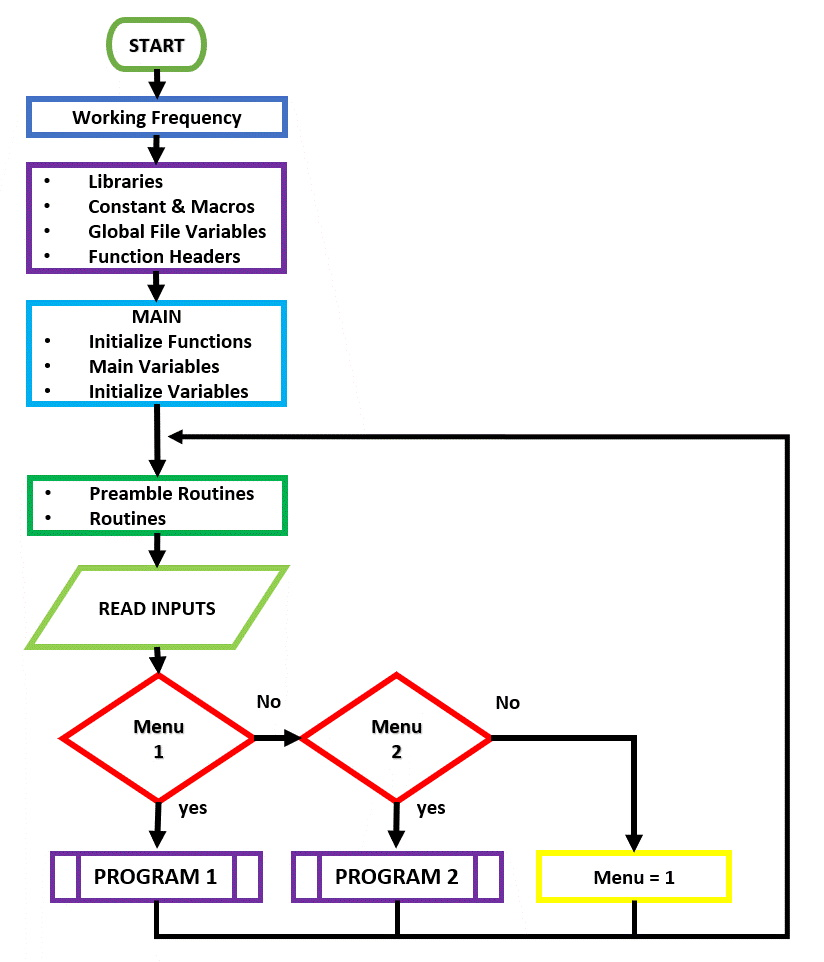
\includegraphics[scale=0.6]{./image/PESTA/flowchart/Main_Program_1.jpg}
	\caption{Estrutura do Programa (fluxograma)}
	\label{Main_Program_1}
\end{figure}
\figurespace{.5}
O \textit{PROGRAM 1} é onde corre o programa da balança, e o \textit{PROGRAM 2} usado para calibração do \textit{gain factor}.
\newpage
Todos os programas seguem uma estrutura sintática recursiva usando o seguinte modelo.
\\
\\
\begin{figure}[H]
	\centering
	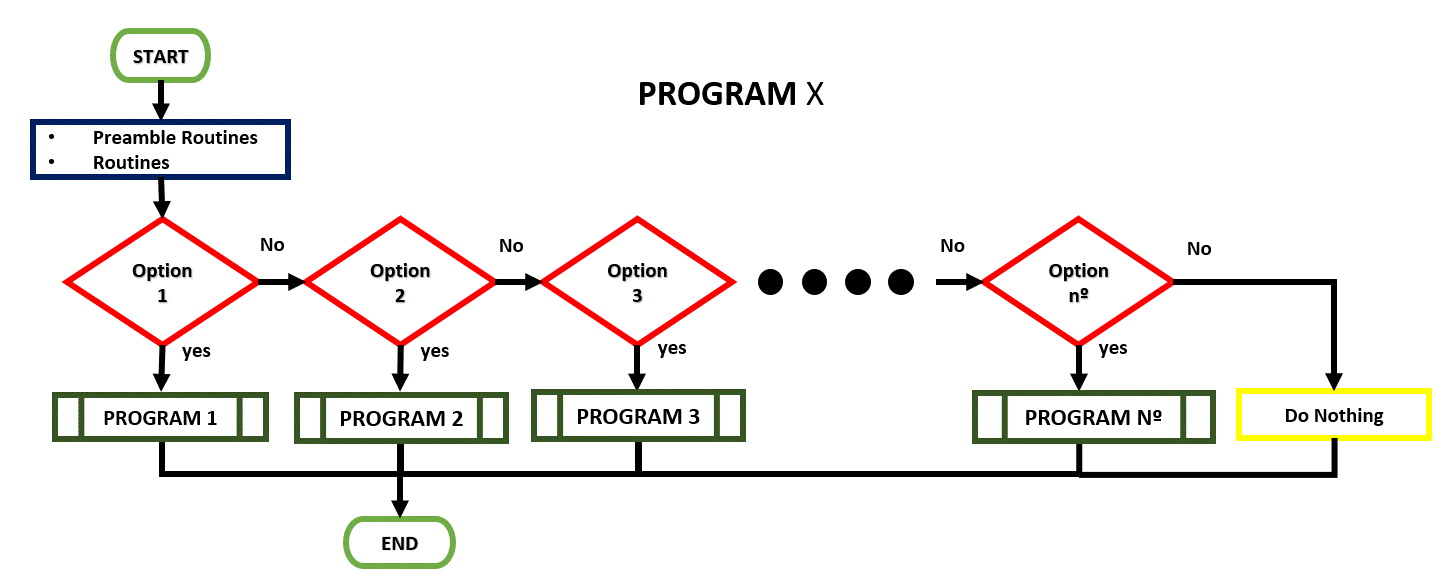
\includegraphics[width=\linewidth]{./image/PESTA/flowchart/Generic_structure.jpg}
	\caption{Sintaxe Genérica dos programas (fluxograma)}
	\label{Geneic_structure}
\end{figure}
\figurespace{.5}
Duas interrupções periódicas estão sempre a correr em \textit{background}, uma para fazer o \textit{shift} dos \textit{bits} da conversão \acs{adc} feita pelo amplificador de sinal HX711 e outra interrupção periódica de segundo em segundo usado para saltar de \textit{Menu} pelos botões.
\\
\\
\begin{minipage}{\linewidth}
\begin{minipage}{.5\linewidth}
\begin{figure}[H]
	\centering
	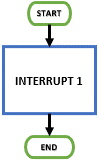
\includegraphics[scale=.85]{./image/PESTA/flowchart/Interrupt_1.jpg}
	\caption{\acs{adc} conversão}
	\label{Interrupt_1}
\end{figure}
\end{minipage}
\begin{minipage}{.5\linewidth}
\begin{figure}[H]
	\centering
	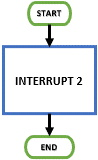
\includegraphics[scale=.85]{./image/PESTA/flowchart/Interrupt_2.jpg}
	\caption{Saltar de \textit{Menu}}
	\label{Interrupt_2}
\end{figure}
\end{minipage}
\end{minipage}
\minipagespace{.5}
Consultar código para leitura das rotinas de interrupção nas folhas \textit{anexas} \ref{main-c}.
\\
\\
\begin{minipage}{.40\linewidth}
\begin{figure}[H]
	\flushleft
	\captionsetup{justification=raggedright,singlelinecheck=false}
	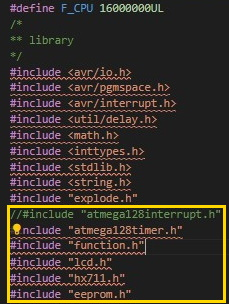
\includegraphics[scale=0.9]{./image/PESTA/Code/Livrarias.jpg}
	\caption{Livrarias}
	\label{Livrarias}
\end{figure}
\end{minipage}
\begin{minipage}{.6\linewidth}
Ao lado esta as livrarias usadas neste projeto, as que estão dentro da caixa amarela são as que foram criadas.
A filosofia usada é de criar objetos que representam o hardware para o poder manipular via código. Como se pode observar foi criado uma livraria para os temporizadores, outra para as interrupções e \ac{eeprom}, depois criado livrarias para os componentes externos, isto é, o \acs{lcd} e o integrado \textbf{HX711}.
\\
Uma abstração que torna simples executar qualquer algoritmo ou projeto, e isto só é possível depois de ultrapassar a barreira de desenvolver as livrarias.
\end{minipage}
\minipagespace{.5}
Durante este projeto tentou-se dentro do possível sempre seguir as boas praticas de programação, como a \texttt{indentação} especifica para cada situação, e manter a estrutura de norma. Deve-se manter uma metodologia de trabalho que segue as normas assim é percetível para todos e facilita detetar \textit{bugs}, e é uma pratica que abrange todas as linguagens, por exemplo o \textbf{Python} é fundado nesse principio.
\\
\\
Quanto as interrupções é sempre um desafio, porque as tarefas tem que ser bem organizadas temporalmente para não entrar em conflitos, pretende-se assim sempre que o código corra na função \textit{main} e as interrupções algo esporádico e muito rápido, estas devem servir de \textit{flags} para executar rotinas na função \textit{main}, ou seja, servirem de \textit{inputs}. %%\textbf{\textcolor{green}{INPUTS}}.
\newpage
%%%%%%%%%%%%%%%%%%%%%%%%%%%%%%%%%%%%%%%%%%%%%%%%%%%%%%%%%%
\section{Validação}
%%%To validate is to justify why the choices made and alternatives that could be chosen.
As escolhas feitas estão dentro dos parâmetros da oferta disponibilizada. Apenas o conhecimento adquirido ao aprofundar o funcionamento dos componentes é o ganho mais evidente, facilitando a interpretação de situações reais e deteção de anomalias (\textit{troubleshooting}), derivado aos custos dos materiais serem caros.
\\
\\
Apostei na marca \textbf{Atmel} devido a experiência e conhecimentos já adquiridos, se aposta-se noutra marca teria de enfrentar uma curva de aprendizagem e adaptação que no final a nível de custos beneficio seria desfavorável, pelo tempo a dispensar e de ser muito trabalhoso ao refazer tudo novamente noutra arquitetura.
\\
\\
O sensor usado é o mais comum nesta pratica, e escolha demonstrada, o circuito de interface é indiferente, a escolha apenas é baseada na sua precisão, ou seja, é de \textcolor{blue}{24} \textit{bits} enquanto o \acs{adc} do \acs{mcu} de apenas \textcolor{blue}{10} \textit{bits} de resolução.
\\
\\
%%%%%%%%%%%%%%%%%%%%%%%%%%%%%%%%%%%%%%%%
\subsection{Material}
Abaixo esta indicado uma tabela dos materiais usados, assim como os preços.
\\
\\
\begin{table}[H]{
		\caption{Lista de material}
		\rowcolors{3}{blue!80!yellow!50}{blue!70!yellow!40}
		\begin{tabular}{ |p{12cm}|c|p{2cm}|  }
			\hline
			\multicolumn{3}{|c|}{Lista de Material} \\
			\hline
			Peça & Quant & Preço [uni] \\
			\hline
			Fonte de alimetação 12V 1A & 1 & \EUR{3.87} \\
			Conversor DC-DC com voltímetro & 1 & \EUR{7.75} \\
			ET BASE AVR Atmega128 Board & 1 & \EUR{23.92} \\
			Test Input Board  & 1 & \EUR{3.71} \\
			Test Output Board & 1 & \EUR{3.71} \\
			\acs{idc} Socket 10 way    & 12 & \EUR{0.31} \\
			\acs{idc} Header Straight 10 way    & 12 & \EUR{0.25} \\
			Flatcable    & ? & \EUR{?} \\
			20x4 \acs{lcd} Module Blue & 1 & \EUR{12.24} \\
			SparkFun Load Cell Amplifier HX711 & 1 & \EUR{13.04}   \\
			50Kg Load Cell & 1 & \EUR{12} \\
			\hline
			& \textit{total} & \EUR{86.96} \\
			\hline
		\end{tabular}
	}
	\label{material}
\end{table}
Os preços são o que estão disponíveis no mercado, quanto a \textit{mainboard} foi o que arranjei com o preço mais competitivo com este \acs{mcu} Atmega 128, outras alternativas atingiam o mesmo preço ou mais caros mas com um \acs{mcu} com menor capacidade.
\newpage
%%%%%%%%%%%%%%%%%%%%%%%%%%%%%%%%%%%%%%%%
\subsection{Testar}
Quanto a funcionalidade no seu todo, a balança tem \textcolor{blue}{quatro} botões e \textcolor{blue}{três} \textit{leds} ativados, um botão para fazer o \textit{offset} no \textcolor{green}{PORTF 0}, e dois botões com dupla função, fazer \textit{reset} para \textit{default} e incrementar, outro para entrar no menu de calibração e decrementar, o \textcolor{blue}{quarto} botão é reservado para \textit{enter} e assumir o valor introduzido na calibração.\\
\\
O botão \textcolor{green}{PORTF 3} quando premido durante \textcolor{blue}{cinco} segundos faz um \textit{reset} para configuração \textit{default} depois de o \textit{led} no \textcolor{red}{PORTC 6} piscar \textcolor{blue}{quatro} vezes.\\
\\
O botão \textcolor{green}{PORTF 4} quando premido durante \textcolor{blue}{cinco} segundos entra no menu de calibração do valor do \textit{gain factor} e o \textit{led} no \textcolor{red}{PORTC 7} liga, usando os botões de incrementa e decrementar, isto é, o
\textcolor{green}{PORTF 3} e \textcolor{green}{PORTF 4} pode-se alterar esse valor.\\
\\
Para assumir o valor e sair do menu de calibração basta premir o botão colocado no \textcolor{green}{PORTF 5}. Tanto no caso de calibração ou de \textit{offset} os valores são guardados na \acs{eeprom} do micro-controlador, sendo que, se retirar a alimentação do circuito este não perde os valores e o \textit{led} \textcolor{red}{PORTC 5} permanece ligado.
\\
\\
%%%%%%%%%%%%%%%%%%%%%%%%%%%%%%%%%%%%%%%%%%%%%%%%%%%%%%%%%%%%%%%%
\begin{comment}
Sem contar com as despesas no equipamento para a programação do hardware que em principio só se gasta uma vez, isto é, se não se estragar. No caso do programador \textbf{Atmel-ICE} pode custar até \EUR{185.55}.\\
\\
É de ter em conta que os preços são \textbf{PVP}, que no caso se for preços comerciais são dez vezes inferior, e se for para produção em grande escala também tem descontos por quantidade.\\
$\begin{array}{l l l}
\text{Média} & & \\
\overline{x} & = & \frac{1}{n}\sum_{i=1}^n x_i
\end{array}$
MEMS devices and structures are fabricated using conventional integrated circuit process techniques, such as lithography, deposition, and etching, together with a broad range of specially developed micromachining techniques. \cite{book-9}\\
The three essential elements in conventional silicon processing are deposition, lithography, and etching. \cite{book-9}\\
Sensitivity, Long-Term Drift and Temperature Effects (Span temperature hysteresis).
\end{comment}
%%%%%%%%%%%%%%%%%%%%%%%%%%%%%%%%%%%%%%%%%%%%%%%%%%%%%%%%%%%%%%%%